\documentclass{standalone}
\usepackage{tikz}
\usetikzlibrary{patterns, positioning}


\begin{document}
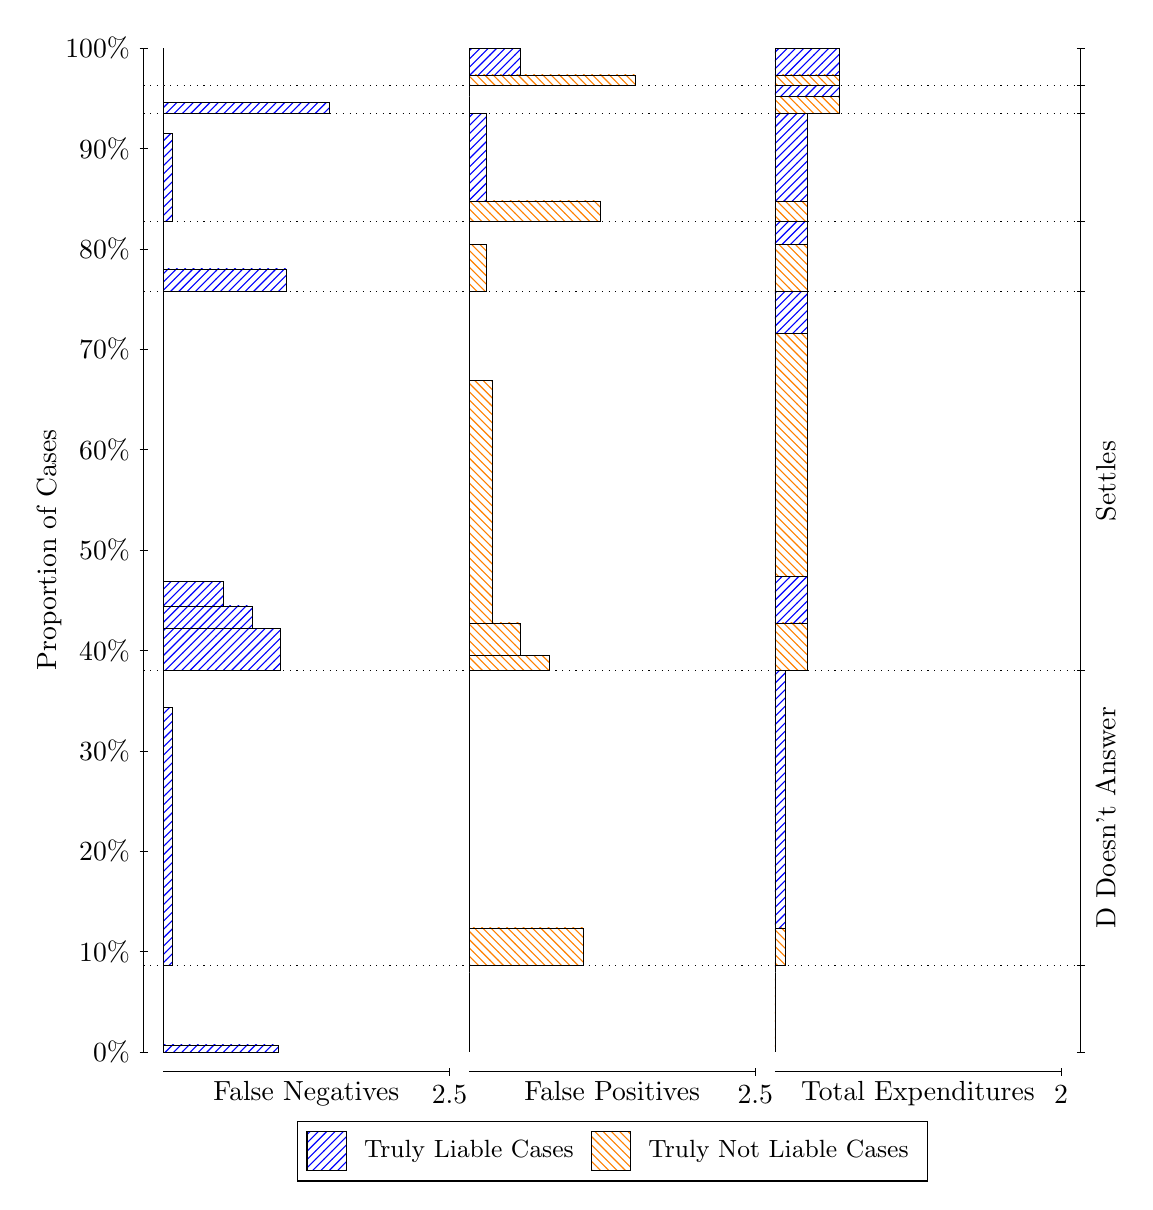
\begin{tikzpicture}
\draw[black, very thin] (1.5,1.75) -- (1.5,14.5);
\node[rotate=90, text=black, anchor=center] at (0.3, 8.125) {Proportion of Cases};
\draw[black, very thin] (1.45,1.75) -- (1.55,1.75);
\node[text=black, anchor=east] at (1.45, 1.75) {0\%};
\draw[black, very thin] (1.45,3.025) -- (1.55,3.025);
\node[text=black, anchor=east] at (1.45, 3.025) {10\%};
\draw[black, very thin] (1.45,4.3) -- (1.55,4.3);
\node[text=black, anchor=east] at (1.45, 4.3) {20\%};
\draw[black, very thin] (1.45,5.575) -- (1.55,5.575);
\node[text=black, anchor=east] at (1.45, 5.575) {30\%};
\draw[black, very thin] (1.45,6.85) -- (1.55,6.85);
\node[text=black, anchor=east] at (1.45, 6.85) {40\%};
\draw[black, very thin] (1.45,8.125) -- (1.55,8.125);
\node[text=black, anchor=east] at (1.45, 8.125) {50\%};
\draw[black, very thin] (1.45,9.4) -- (1.55,9.4);
\node[text=black, anchor=east] at (1.45, 9.4) {60\%};
\draw[black, very thin] (1.45,10.675) -- (1.55,10.675);
\node[text=black, anchor=east] at (1.45, 10.675) {70\%};
\draw[black, very thin] (1.45,11.95) -- (1.55,11.95);
\node[text=black, anchor=east] at (1.45, 11.95) {80\%};
\draw[black, very thin] (1.45,13.225) -- (1.55,13.225);
\node[text=black, anchor=east] at (1.45, 13.225) {90\%};
\draw[black, very thin] (1.45,14.5) -- (1.55,14.5);
\node[text=black, anchor=east] at (1.45, 14.5) {100\%};

\draw[black, very thin] (13.4,1.75) -- (13.4,14.5);
\draw[black, very thin] (13.35,1.75) -- (13.45,1.75);
\node[anchor=west] at (13.35, 1.75) {};
\draw[black, very thin] (13.35,2.8498) -- (13.45,2.8498);
\node[anchor=west] at (13.35, 2.8498) {};
\draw[black, very thin] (13.35,6.5973) -- (13.45,6.5973);
\node[anchor=west] at (13.35, 6.5973) {};
\draw[black, very thin] (13.35,11.406) -- (13.45,11.406);
\node[anchor=west] at (13.35, 11.406) {};
\draw[black, very thin] (13.35,12.295) -- (13.45,12.295);
\node[anchor=west] at (13.35, 12.295) {};
\draw[black, very thin] (13.35,13.674) -- (13.45,13.674);
\node[anchor=west] at (13.35, 13.674) {};
\draw[black, very thin] (13.35,14.021) -- (13.45,14.021);
\node[anchor=west] at (13.35, 14.021) {};
\draw[black, very thin] (13.35,14.5) -- (13.45,14.5);
\node[anchor=west] at (13.35, 14.5) {};

\draw[black, very thin, pattern color=blue, pattern=north east lines] (1.75,1.75) rectangle (3.2033,1.839);
\draw[black, very thin, pattern color=orange, pattern=north west lines] (1.75,1.839) rectangle (1.75,2.8498);
\draw[black, very thin, pattern color=blue, pattern=north east lines] (1.75,2.8498) rectangle (1.859,6.1221);
\draw[black, very thin, pattern color=orange, pattern=north west lines] (1.75,6.1221) rectangle (1.75,6.5973);
\draw[black, very thin, pattern color=blue, pattern=north east lines] (1.75,6.5973) rectangle (3.2397,7.1318);
\draw[black, very thin, pattern color=blue, pattern=north east lines] (1.75,7.1318) rectangle (2.8763,7.4157);
\draw[black, very thin, pattern color=blue, pattern=north east lines] (1.75,7.4157) rectangle (2.513,7.7249);
\draw[black, very thin, pattern color=orange, pattern=north west lines] (1.75,7.7249) rectangle (1.75,11.406);
\draw[black, very thin, pattern color=blue, pattern=north east lines] (1.75,11.406) rectangle (3.3123,11.696);
\draw[black, very thin, pattern color=orange, pattern=north west lines] (1.75,11.696) rectangle (1.75,12.295);
\draw[black, very thin, pattern color=blue, pattern=north east lines] (1.75,12.295) rectangle (1.859,13.412);
\draw[black, very thin, pattern color=orange, pattern=north west lines] (1.75,13.412) rectangle (1.75,13.674);
\draw[black, very thin, pattern color=blue, pattern=north east lines] (1.75,13.674) rectangle (3.8573,13.813);
\draw[black, very thin, pattern color=orange, pattern=north west lines] (1.75,13.813) rectangle (1.75,14.021);
\draw[black, very thin, pattern color=orange, pattern=north west lines] (1.75,14.021) rectangle (1.75,14.159);
\draw[black, very thin, pattern color=blue, pattern=north east lines] (1.75,14.159) rectangle (1.75,14.5);
\draw[black, very thin, pattern color=orange, pattern=north west lines] (5.6333,1.75) rectangle (5.6333,2.7608);
\draw[black, very thin, pattern color=blue, pattern=north east lines] (5.6333,2.7608) rectangle (5.6333,2.8498);
\draw[black, very thin, pattern color=orange, pattern=north west lines] (5.6333,2.8498) rectangle (7.0867,3.3251);
\draw[black, very thin, pattern color=blue, pattern=north east lines] (5.6333,3.3251) rectangle (5.6333,6.5973);
\draw[black, very thin, pattern color=orange, pattern=north west lines] (5.6333,6.5973) rectangle (6.6507,6.7902);
\draw[black, very thin, pattern color=orange, pattern=north west lines] (5.6333,6.7902) rectangle (6.2873,7.1992);
\draw[black, very thin, pattern color=orange, pattern=north west lines] (5.6333,7.1992) rectangle (5.924,10.279);
\draw[black, very thin, pattern color=blue, pattern=north east lines] (5.6333,10.279) rectangle (5.6333,11.406);
\draw[black, very thin, pattern color=orange, pattern=north west lines] (5.6333,11.406) rectangle (5.8513,12.006);
\draw[black, very thin, pattern color=blue, pattern=north east lines] (5.6333,12.006) rectangle (5.6333,12.295);
\draw[black, very thin, pattern color=orange, pattern=north west lines] (5.6333,12.295) rectangle (7.3047,12.558);
\draw[black, very thin, pattern color=blue, pattern=north east lines] (5.6333,12.558) rectangle (5.8513,13.674);
\draw[black, very thin, pattern color=orange, pattern=north west lines] (5.6333,13.674) rectangle (5.6333,13.882);
\draw[black, very thin, pattern color=blue, pattern=north east lines] (5.6333,13.882) rectangle (5.6333,14.021);
\draw[black, very thin, pattern color=orange, pattern=north west lines] (5.6333,14.021) rectangle (7.7407,14.159);
\draw[black, very thin, pattern color=blue, pattern=north east lines] (5.6333,14.159) rectangle (6.2873,14.5);
\draw[black, very thin, pattern color=orange, pattern=north west lines] (9.5167,1.75) rectangle (9.5167,2.7608);
\draw[black, very thin, pattern color=blue, pattern=north east lines] (9.5167,2.7608) rectangle (9.5167,2.8498);
\draw[black, very thin, pattern color=orange, pattern=north west lines] (9.5167,2.8498) rectangle (9.6529,3.3251);
\draw[black, very thin, pattern color=blue, pattern=north east lines] (9.5167,3.3251) rectangle (9.6529,6.5973);
\draw[black, very thin, pattern color=orange, pattern=north west lines] (9.5167,6.5973) rectangle (9.9254,7.1992);
\draw[black, very thin, pattern color=blue, pattern=north east lines] (9.5167,7.1992) rectangle (9.9254,7.7923);
\draw[black, very thin, pattern color=orange, pattern=north west lines] (9.5167,7.7923) rectangle (9.9254,10.872);
\draw[black, very thin, pattern color=blue, pattern=north east lines] (9.5167,10.872) rectangle (9.9254,11.406);
\draw[black, very thin, pattern color=orange, pattern=north west lines] (9.5167,11.406) rectangle (9.9254,12.006);
\draw[black, very thin, pattern color=blue, pattern=north east lines] (9.5167,12.006) rectangle (9.9254,12.295);
\draw[black, very thin, pattern color=orange, pattern=north west lines] (9.5167,12.295) rectangle (9.9254,12.558);
\draw[black, very thin, pattern color=blue, pattern=north east lines] (9.5167,12.558) rectangle (9.9254,13.674);
\draw[black, very thin, pattern color=orange, pattern=north west lines] (9.5167,13.674) rectangle (10.334,13.882);
\draw[black, very thin, pattern color=blue, pattern=north east lines] (9.5167,13.882) rectangle (10.334,14.021);
\draw[black, very thin, pattern color=orange, pattern=north west lines] (9.5167,14.021) rectangle (10.334,14.159);
\draw[black, very thin, pattern color=blue, pattern=north east lines] (9.5167,14.159) rectangle (10.334,14.5);
\draw[black, dotted] (1.5,2.8498) -- (13.4,2.8498);
\draw[black, dotted] (1.5,6.5973) -- (13.4,6.5973);
\draw[black, dotted] (1.5,11.406) -- (13.4,11.406);
\draw[black, dotted] (1.5,12.295) -- (13.4,12.295);
\draw[black, dotted] (1.5,13.674) -- (13.4,13.674);
\draw[black, dotted] (1.5,14.021) -- (13.4,14.021);
\draw[black, very thin] (1.75,1.5) -- (5.3833,1.5);
\node[text=black, anchor=north] at (3.5667, 1.5) {False Negatives};
\draw[black, very thin] (5.3833,1.45) -- (5.3833,1.55);
\node[text=black, anchor=north] at (5.3833, 1.45) {2.5};

\draw[black, very thin] (5.6333,1.5) -- (9.2667,1.5);
\node[text=black, anchor=north] at (7.45, 1.5) {False Positives};
\draw[black, very thin] (9.2667,1.45) -- (9.2667,1.55);
\node[text=black, anchor=north] at (9.2667, 1.45) {2.5};

\draw[black, very thin] (9.5167,1.5) -- (13.15,1.5);
\node[text=black, anchor=north] at (11.333, 1.5) {Total Expenditures};
\draw[black, very thin] (13.15,1.45) -- (13.15,1.55);
\node[text=black, anchor=north] at (13.15, 1.45) {2};


\node[text=black, centered, rotate=90] at (13.72, 4.7236) {D Doesn't Answer};
\node[text=black, centered, rotate=90] at (13.72, 9.0018) {Settles};





\draw (7.449999999999999,1.5) node[draw=none] (baseCoordinate) {};
\begin{scope}[align=center]
        \matrix[scale=0.5, draw=black, below=0.5cm of baseCoordinate, nodes={draw}, column sep=0.1cm]{
            \node[rectangle, draw, minimum width=0.5cm, minimum height=0.5cm, pattern color=blue, pattern=north east lines] {}; &
            \node[draw=none, font=\small, text=black] (B) {Truly Liable Cases}; &
            \node[rectangle, draw, minimum width=0.5cm, minimum height=0.5cm, pattern color=orange, pattern=north west lines] {}; &
            \node[draw=none, font=\small, text=black] (B) {Truly Not Liable Cases}; \\
            };
\end{scope}

\end{tikzpicture}
\end{document}